\documentclass{scrreprt}

\usepackage{aligned-overset}
\usepackage{amsmath}
\usepackage{amssymb}
\usepackage{bm}
\usepackage[shortlabels]{enumitem}
\usepackage{hyperref}
\usepackage[utf8]{inputenc}
\usepackage{mathtools}
\usepackage{physics}
\usepackage{tabularx}
\usepackage{titling}
\usepackage{fancyhdr}
\usepackage{xfrac}
\usepackage{pgfplots}

\definecolor{light-gray}{gray}{.9}

\pgfplotsset{compat = newest}
\usetikzlibrary{intersections}
\usetikzlibrary{patterns}
\usepgfplotslibrary{fillbetween}

\author{Karsten Lehmann}
\date{SoSe 2021}
\title{Übung 05 Analysis - Weiterführende Konzepte}

\pagestyle{fancy}
\fancyhf{}
\lhead{\thetitle}
\rhead{\theauthor}
\lfoot{\thedate}
\rfoot{Seite \thepage}

\begin{document}

\section*{Stetigkeit und kompakte Mengen in metrischen Räumen}

Skizzieren Sie die folgenden Mengen $K \in \mathbb{R}^2$.
Untersuchen Sie, ob die angegebenen Funktionen $f: K \to \mathbb{R}$
Minimum und Maximum auf $K$ besitzen.
\begin{enumerate}[(i)]
\item $K \coloneqq \qty{x = \qty(x_1, x_2) \in \mathbb{R}^2 \middle|
    (x_1, x_2 \geq 0) \land (2x_1 + x_2 \leq 3)}$ und
  $f\qty(x_1, x_2) \coloneqq \sin\qty(x_1 \cdot x_2) \cdot
  \ln\qty(\frac{1 + x_1}{2 + x_2^2})$

  \textit{Lsg.} Aus den Beschränkungen für $x_1$ und $x_2$ folgt
  \[
    0 \leq x_1 \leq \frac{1}{2}\qty(3- x_2) \leq \frac{3}{2}
    \text{ und }
    0 \leq x_2 \leq 3 - 2x_1 \leq 3
  \]
  $\Rightarrow K \subseteq A \coloneqq [0, 3] \times [0, 3]
  \Rightarrow K$ ist beschränkt.

  \begin{center}
    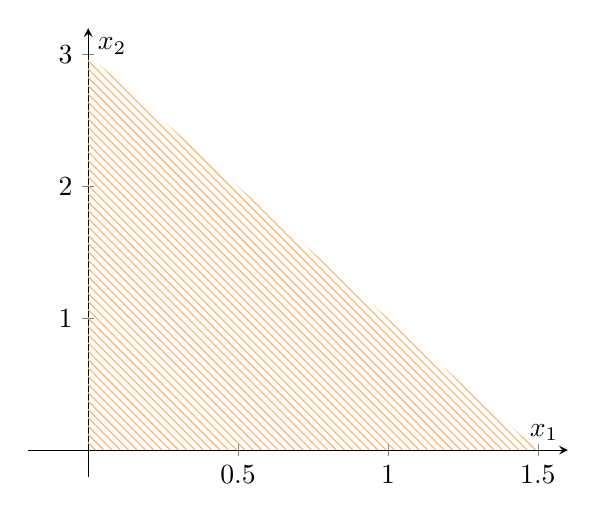
\begin{tikzpicture}
      \begin{axis}[
        axis lines=middle,
        xlabel=$x_1$,
        xmax = 1.6,
        xmin = -0.2,
        ylabel=$x_2$,
        ymax = 3.2,
        ymin = -0.2,
      ]
        \addplot[draw=none, pattern color=orange!60, pattern=north west lines] coordinates
        {(0, 0) (0, 3) (1.5, 0)};
      \end{axis}
    \end{tikzpicture}
  \end{center}
  Die Funktionen $g(x_1, x_2) \coloneqq x_1$, $h(x_1, x_2) \coloneqq x_2$,
  $j(x_1, x_2) \coloneqq 2x_1 + x_2$ sind stetig.

  Die Urbilder abgeschlossener Mengen
  \begin{flalign*}
    A_1 &= g^{-1}([0, \infty)) = [0, \infty) \times \mathbb{R} & \\
    A_2 &= h^{-1}([0, \infty)) = \mathbb{R} \times [0, \infty) \\
    A_3 &= j^{-1}((-\infty, 3]) = \qty{(x_1, x_2) \in \mathbb{R}^2 \middle|
      (x_1 \in \mathbb{R}) \land (x_2 \leq 3 - 2x_1)}
  \end{flalign*}
  sind somit abgeschlossen und
  $K = A_1 \cap A_2 \cap A_3$ ist ebenfalls abgeschlossen.
  Weiterhin ist $f$ als Komposition stetiger Funktionen ebenfalls stetig
  und es existieren Punkte $a = (a_1, a_2), b = (b_1, b_2) \in \mathbb{R}^2$
  mit $f(a) \leq f(x) \leq f(b) \forall x \in K$.

\newpage
\item $K \coloneqq \qty{x = \qty(x_1, x_2) \in \mathbb{R}^2 \middle|
    \abs{x_1 \cdot x_2} \leq 1}$ und
  $f\qty(x_1, x_2) \coloneqq \sin(x_1) + \abs{x_2}$ \\

  \textit{Lsg.}
  \begin{flalign*}
    K &= \qty{(x_1, x_2) \in \mathbb{R}^2 \middle|
         x_1 = 0 \lor x_2 \leq \frac{1}{\abs{x_1}}} & \\
      &= \qty(\bigcup_{x_1 \ne 0} \qty{x_1} \times
         \qty[-\frac{1}{\abs{x_1}}, \frac{1}{\abs{x_1}}])
         \cup \qty{\qty{0} \times \mathbb{R}}
   \end{flalign*}
   $\Rightarrow K$ ist nicht beschränkt $K$ ist nicht kompakt.

   \begin{center}
     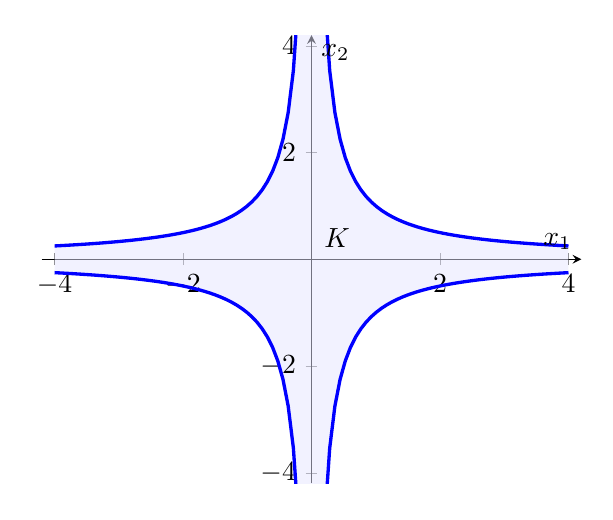
\begin{tikzpicture}[
         declare function={
           f(\x) = \x != 0 ? 1 / abs(\x) : 5;
         }
       ]
       \begin{axis}[
         axis lines=middle,
         xlabel=$x_1$,
         xmax = 4.2,
         xmin = -4.2,
         ylabel=$x_2$,
         ymax = 4.2,
         ymin = -4.2,
       ]
         \addplot[
           domain = -4:4,
           very thick,
           name path = f1,
           samples = 100,
           blue,
         ] {f(x)};
         \addplot[
           domain = -4:4,
           very thick,
           name path = f2,
           samples = 100,
           blue,
         ] { -1 *  f(x)};
         \addplot[
           fill = blue!10,
           fill opacity = .5,
         ] fill between[of = f1 and f2];
         \node at (.4,.4) {$K$};
       \end{axis}
     \end{tikzpicture}
   \end{center}

   Auch $f$ ist wegen $f(0, x_2) = \abs{x_2}, x_2 \in \mathbb{R}$
   nicht nach oben beschränkt.
   $\Rightarrow f$ besitzt kein Maximum oder Supremum auf $K$.

  \begin{minipage}[t]{.45\textwidth}
    \textbf{Fall 1}: $x_1 = 0$:
    \[
      f(x_1, x_2) = \abs{x_2} \geq 0, x_2 \in \mathbb{R}
    \]
  \end{minipage}
  \vrule
  \hfill
  \begin{minipage}[t]{.45\textwidth}
    \textbf{Fall 2}: $x_2 = 0$
    \begin{align*}
      f{x_1, x_2} &= \sin(x_1) + \abs{x_2} \geq \sin(x_1) \\
                  &= f(x_1, 0) \geq -1 \\
                  &= f\qty(2k\pi + \frac{3}{2}\pi, 0), k \in \mathbb{Z}
    \end{align*}
  \end{minipage} \\

  $f$ besitzt auf $K$ das Minimum $-1$

\end{enumerate}

\newpage
\noindent
Gegeben seien ein metrischer Raum $(M, d)$ und nichtleere Teilmengen
$A, K \subseteq M$.
\begin{enumerate}[a)]
\item Beweisen Sie die sogenannte Vierecksungleichung:
  Für $x, y, u, v \in M$ gilt
  \[
    \abs{d(x, y) - d(u, v)} \leq d(x, u) + d(y, v)
  \]
  \textit{Lsg.} Nach der Dreiecksungleichung ist
  \begin{align*}
    d(x, y) &\leq d(x, u) + d(y, u) \leq d(x, u) + d(u, v) + d(v, y) \\
            &\Rightarrow d(x, y) - d(u, v) \leq d(x, u) + d(y, v) \\
    d(u, v) &\leq d(u, x) + d(v, x) \leq d(x, u) + d(x, y) + d(y, v) \\
            &\Rightarrow -1 \cdot (d(x, y) - d(u, v)) \leq d(x, u) + d(y, v) \\
            &\Rightarrow \abs{d(x, y) - d(u, v)} \leq d(x, u) + d(y, v)
  \end{align*}

\item $M \times M$ sei mit der Metrik
  $\hat{d}((x, y), (u, v)) = d(x, u) + d(y, v)$ versehen.
  Beweisen Sie, dass die Abbildung $d \colon M \times M \to \mathbb{R}$
  stetig ist.

  \textit{Lsg.} seien $(x, y) \in M \times M$ ein Punkt und
  $\qty(x_n), \qty(y_n)$ zwei Folgen mit
  $x_n \overset{n \to \infty}\longrightarrow x$ und
  $y_n \overset{n \to \infty}\longrightarrow y$.
  Aus $a)$ folgt
  \[
    \abs{d(x, y) - d(x_n, y_n)} \leq d(x, x_n) + d(y, y_n)
    \overset{n \to \infty}\longrightarrow 0
  \]
  Folglich ist $d$ stetig in $(x, y) \in M \times M$.
  Da $(x, y)$ beliebig ist, ist $d$ auf $M \times M$ stetig.

\item Beweisen Sie, dass durch
  $f(x) \coloneqq d(x, A) \coloneqq \underset{y \in A}\inf d(x, y)$
  eine Lipschitz-stetige Abbildung $f \colon M \to \mathbb{R}$
  definiert ist.

  \textit{Lsg.} Seien $a, b \in M$ gegeben.
  Dann gilt für $c \in A$:
  \begin{align*}
    f(a) &= \underset{y \in A}\inf d(a, y) \leq d(a, c) \leq d(a, b) + d(b, c) \\
    f(a) &\leq \underset{c \in A}\inf \qty(d(a, b) + d(b, c)) = d(a, b) + \inf \leq d(a, b) + f(b) \\
    \abs{f(a) - f(b)} &\leq d(a, b) \Rightarrow f \text{ ist Lipschitzstetig mit $L = 1$}
  \end{align*}

\item Sei $g(A, K) \coloneqq \underset{(x, y) \in A \times K}\inf d(x, y)$.
  Zeigen Sie: Ist $A \subseteq M$ abgeschlossen und $K \subseteq M$ kompakt
  mit $A \cap K = \emptyset$, so gilt $g(A, K) > 0$.

  \textit{Lsg.} Angenommen $g(A, K) = 0$.
  Dann existieren Folgen $\qty(a_n)$ in $A$ und $\qty(b_n)$ in $K$
  mit $d\qty(a_n, b_n) \overset{n \to \infty}\longrightarrow g(A, K) = 0$
  Aus der Kompaktheit von $K$ folgt die Existenz einer in $K$
  konvergenten Teilfolge $\qty(b_{n_k})$ mit
  $b_{n_k} \overset{k \to \infty}\longrightarrow b \in K$.
  Jetzt ist $d\qty(b, a_{n_k}) \leq d\qty(b, b_{n_k}) + d(a_{n_k}, b_{n_k})
  \overset{k \to \infty}\longrightarrow 0$.
  Da $A$ abgeschlossen ist, muss nun $b \in A \cap K = \emptyset$ sein,
  ein Widerspruch.

\item Geben Sie Beispiele abgeschlossener,disjunkter Mengen $A, B$ aus
  $\mathbb{R}$ bzw. $\mathbb{R}^2$ an, deren Abstand $g(A, K) = 0$ ist.

  \textit{Lsg.} In $\mathbb{R}$: $A \coloneqq \qty{n \middle| n \in \mathbb{N}}$
  und $B \coloneqq \qty{n + \frac{1}{n} \middle| n \in \mathbb{N}}$ \\
  In $\mathbb{R}^2$ : $A \coloneqq \qty{(x, 0) \middle| x \in \mathbb{R}}$
  und $B \coloneqq \qty{(x, y) \middle| x \in \mathbb{R} \land y \geq e^x}$
\end{enumerate}

\newpage
\noindent
Gegeben seien ein vollständiger metrischer Raum $(M, d)$, eine Folge
abgeschlossener Kugeln $B_n \coloneqq B\qty[x_n, \epsilon_n]$ mit
$x_n \in M, \epsilon_n > 0$, so dass $B_{n + 1} \subseteq B_n$ und
$\lim_{n \to \infty} \epsilon_n = 0$ gilt.

Beweisen Sie, dass der Durchschnitt $\underset{n \in \mathbb{N}}\bigcap B_n$
nichtleer ist und genau ein Element enthält.

\textit{Lsg.} Für $n \in \mathbb{N}$ und $m \leq n$ gilt
$x_m \in B_n$, dass heißt $d(x_n, x_m) < \epsilon_n$.
Sei $\epsilon > 0$ gegeben, dann existiert wegen
$\lim_{n \to \infty} \epsilon_n = 0$ ein $n_0 \in \mathbb{N}$ mit
$\epsilon_{n_0} < \frac{\epsilon}{2}$.
Für $m, n \geq n_0$ folgt
\[
  d(x_n, m_m) \leq d\qty(x_n, x_{n_0}) + d\qty(x_{n_0}, x_m) < 2 \epsilon_{n_0} < \epsilon
\]
$\Rightarrow \qty(x_n)$ ist eine Cauchy-Folge.
Da $M$ vollständig ist, existiert $x_n \overset{n \to \infty}\longrightarrow x$
und $B$ ist als Durchschnitt abgeschlossener Kugeln abgeschlossen.
Somit ist $x \in B$.

Sei nun $y \ne x \in B$.
Dann ist $\epsilon \coloneqq d(x, y) > 0$.
Wegen $\lim_{n \to \infty} \epsilon_n = 0$ ein $n_0 \in \mathbb{N}$ mit
$\epsilon_{n_0} < \frac{\epsilon}{2}$.
Wegen $x, y \in B_n$ gilt für $n \geq n_0$
\[
  d(x, y) \leq d(x, x_n) + d(x_n, y) < 2 \epsilon_{n_0} < \epsilon
\]
ein Widerspruch.

\end{document}